\begin{framed}\noindent
	
	\textbf{Bài 3 - Bài toán đề nghị tháng 8/2018 - Phan Quang Trí}
	
	Cho tam giác $\triangle ABC$ nội tiếp đường tròn $(O)$. Gọi $X, Y$ lần lượt là trung điểm $CA, AB$. Gọi $K = AO \cap BC$. Gọi $E, F$ lần lượt là tâm của $(AXK), (AYK)$. Chứng minh $YE, XF$ cắt nhau trên tiếp tuyến tại $A$ của $(O)$.
	
\end{framed}

\textbf{Lời giải 1 - Nguyễn Duy Khang.}

\begin{center}
	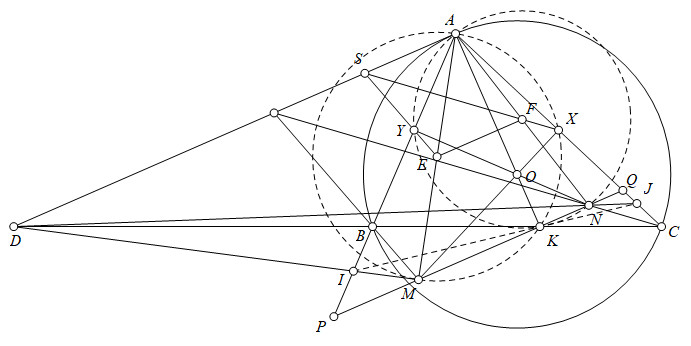
\includegraphics[scale=0.6]{T082018/T82018_TriPQ_SOL2}
	
\end{center}

Kẻ đường kính $AM$ của $(AXK)$ và đường kính $AN$ của $(AYK)$. Ta sẽ chứng minh: $BM, CN$ cắt nhau trên tiếp tuyến tại $A$ của $(O)$. Dễ dàng nhận thấy một số điều sau: $M, O, X$ thẳng hàng, $N, O, Y$ thẳng hàng, $M, K, N$ thẳng hàng, tứ giác $MNXY$ nội tiếp, tứ giác $PQXY$ nội tiếp. Từ đó, ta có: $\angle MYP = \angle NXQ$.

Giả sử tiếp tuyến tại $A$ của $(O)$ cắt $BC$ tại $D$, theo định lý Desargues cho hai tam giác $DMN$ và $ABC$: $BM, CN, AD$ đồng quy khi và chỉ khi $I = DM \cap AB, K = MN \cap BC, J = DN \cap AC$ thẳng hàng.

Thật vậy, theo định lý \textit{Menelaus} thì ta chỉ cần chứng minh: $ \dfrac{IM}{ID}.\dfrac{JD}{JN}.\dfrac{KN}{KM} = 1$.

Biến đổi vế trái, ta có: 

$ \dfrac{IM}{ID}.\dfrac{JD}{JN}.\dfrac{KN}{KM} = \dfrac{MP}{DA}.\dfrac{DA}{NQ}.\dfrac{ON cos{\angle ONK}}{OM cos {\angle OMK}}$

$= \dfrac{MP}{NQ}.\dfrac{ON}{OM}.\dfrac{cos{\angle ONK}}{cos {\angle OMK}}$ = $= \dfrac{MP}{NQ}.\dfrac{NX}{MY}.\dfrac{sin{\angle MPY}}{sin{\angle NQX}} = \dfrac{MP}{MY}.\dfrac{NX}{NQ}.\dfrac{sin{\angle MPY}}{sin{\angle NQX}}$

$= \dfrac{sin{\angle MYP}}{sin{\angle MPY}}.\dfrac{sin{\angle NQX}}{sin{\angle NXQ}}.\dfrac{sin{\angle MPY}}{sin{\angle NQX}} = 1$.

Suy ra đpcm. Tới đây xét phép vị tự tâm $A$ tỉ số $\dfrac{1}{2}$ biến $BM$ thành $YE$, biến $CN$ thành $XF$, biến tiếp tuyến tại $A$ của $(O)$ thành chính nó. Do $BM, CN, AD$ đồng quy nên $YE, XF, AD$ cũng đồng quy. $\qquad \blacksquare$

\textbf{Lời giải 2 - Nguyễn Duy Hiếu.}

\begin{center}
	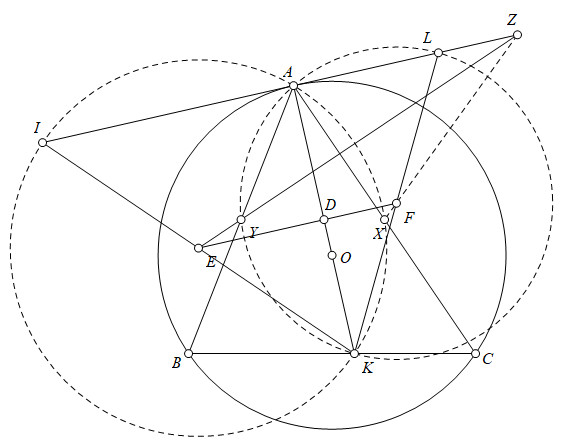
\includegraphics[scale=0.6]{T082018/T82018_TriPQ_SOL3}
	
\end{center}

Kẻ các đường kính $KI$ và $KL$ của $(E)$ và $(F)$, suy ra $IL$ là tiếp tuyến của $(A)$. Gọi $D$ là trung điểm $AK$ thì $XY$ và $EF$ đều đi qua $D$. Gọi $Z$ là giao của $YE$ với $IL$. Ta có:

$$ \dfrac{ZE}{ZY} = \dfrac{d(E,IL)}{d(Y,IL)} = \dfrac{\dfrac{1}{2}AK}{AY sin{\angle IAY}} = \dfrac{AK}{AB sinC} = \dfrac{CK}{AB sin{\angle KAC}}$$.

$$ \dfrac{XY}{XD} = \dfrac{CB}{CK}$$

$$ \dfrac{ZE}{ZY}.\dfrac{XY}{XD} = \dfrac{CB}{AB sin{\angle KAC}} = \dfrac{sinA}{sinC.cosB}$$.

Để ý: $\triangle YAL \sim \triangle YOK$ (g-g) nên $\dfrac{AL}{OK} = \dfrac{YA}{YO} = tan{\angle AOY} = tan C$. Tương tự, ta cũng có: $\dfrac{AI}{OK} = tanB$ nên $$ \dfrac{DF}{DE} = \dfrac{AL}{AI} = \dfrac{tanC}{tanB} = \dfrac{cosBsinC}{sinBcosC}$$.

$$ \Longrightarrow \frac{FD}{FE} = \dfrac{cosBsinC}{sinBcosC+cosBsinC} = \dfrac{cosBsinC}{sin(B+C)} = \dfrac{cosBsinC}{sinA}$$.

Từ đó ta có: $\dfrac{ZE}{ZY}.\dfrac{XY}{XD}.\dfrac{FD}{FE} = 1$ hay $Z, X, F$ thẳng hàng, suy ra $XF$ cắt $YE$ tại $Z$ nằm trên $IL$ là tiếp tuyến tại $A$ của $(O)$. Kết thúc chứng minh. $\qquad \blacksquare$